\chapter{Introduction}
\label{chap:intro}
In this chapter, we first briefly introduce the background of the research on human mobility as well as the corresponding visualization. Then we summarize the data source that are used to describe the human movement. After that, we summarize the general tasks of the human mobility analysis. At last, an overview of the whole survey is given.


\section{Background}

Movement is the fundamental characteristics of all the species, especially for the human-being, the movement range greatly represents the evolution history as well as the development of society and technology, while the movement patterns can also reflect the activities in relative small scale. Especially in the recent 150 years, with the rapid development of modern traffic, the movement pattern tends to be more diversified and complicated.  With the advanced sensing and location-based technology, more and more movement data are captured to describe human’s mobility. Nowadays, the movement data could precisely describe human activities in the urban, and raise an increasing attention of researchers in different research domains like urbanology, meteorology, sociology and economics. 

However, the analysis of the movement data is difficult, in addition to the increasing data size, the movement data has spatial-temporal features which is independent to other attributes. And the movement patterns also differ from time and region. Besides, some reasoning tasks from the data are also require domain knowledge, which needs the involvement of domain expert. 

Visualization provides the methods that leverage the distinct capabilities of machine and human for the exploration tasks. Hundreds of years ago, the visualization to human movement has been designed that enable human to understand the movement patterns. 

A classic case of the mobility visualization is Napoleon’s campaign to Russia(Figure ~\ref{fig:napoleon}) which is depicted by French civil engineer Charles Joseph Minard. This well designed figure not only the present the spatial-temporal features of the marching route, but also the moving directions, number of troops as well as the temperature.  


\begin{figure}[!htb]
  \centering
  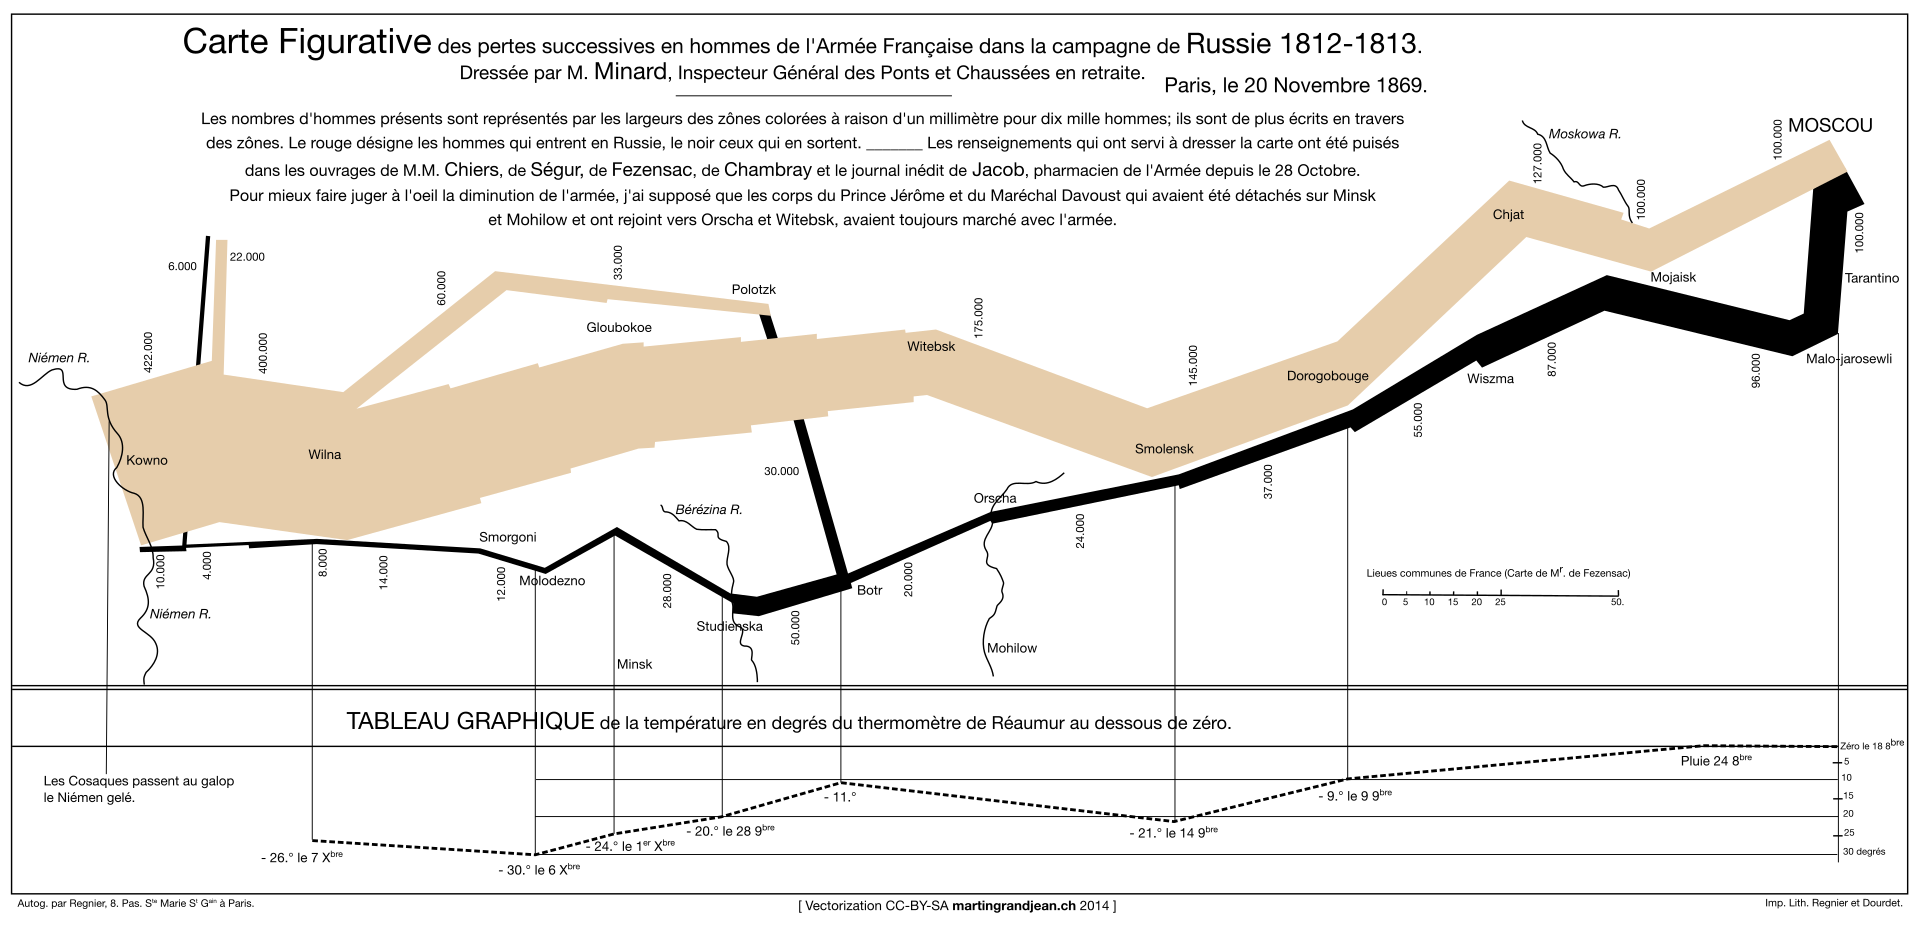
\includegraphics[width = 400px]{figures/Napoleon_war.png}
  \caption{Charles Minard's map of Napoleon’s campaign to Russia of 1812. The band illustrates the marching route from Kaunas to Moscow. The position on the figure present the relative position of geo-map. The band width illustrates the troop number and the color indicates the directions of departure and withdraw. }
  \label{fig:napoleon}
\end{figure}

With the rapid development of computer techniques, the more advanced visual analytics are designed based on powerful computing capability as well as the efficient algorithms. Instead the effectiveness of visual design, the modern visual analytics also focus on the how to bridge the gap between users and computers. As for the exploration itself, the interactive analysis on complicated tasks should be considered. 

\section{Data classification}

Nowadays, with the development of sensing technology, more and more types of data reflecting the human movement can be collected. The variety type of data enables researchers to analyze the human mobility from different perspective and granularity. Here we summarize the data into the following categories according to the characteristic, these characteristic highly related to how the data are collected: 

\textbf{Data collected by professional location device:} Including the vehicle trajectory\cite{liu2017smartadp}, aircraft trajectory\cite{lampe2011interactive} and the vessel trajectory\cite{willems2009visualization}. This kind of movement data is commonly collected by professional location devices which can provide continuous and fine-grained position records. For example, most taxis are equipped with GPS device, a set of discrete location points are generated and recorded. Due to the fine spatial continuity, this type of data can meet the study of different granularity.

\textbf{Data collected by the device with fixed position:} Some devices cannot generate position information by themselves, however, when  pass through specific regions or devices, the locations can be recorded, this type of data provides a chance to analyze the human mobility among the fixed regions or devices. For example, the using of public bicycle in London\cite{wood2011visualizing}, when users hire or release bicycle, the records will be generated by docking stations. This is similar to the metro ticketing\cite{itoh2016visual} data and the traffic monitoring data\cite{guo2011tripvista}. Another special case is the mobile phone using data. The location of mobile phone can be recorded through the mobile stations. Even through the triangle localization, the relative accurate location can be calculated, however, due to some practical issue, the movement of mobile phone is always analyzed among the stations\cite{wu2016telcovis}. In summary, this type of data always analyzed in a way of origin-destination which will be discussed in detail in the Chapter 4. 

\textbf{Data collected by software on mobile device:} More and more people today rely on social media to post their status or connect friends. When messages are post on the social media platform, the position information is also located. The social media provides a more sparse way to record the movement of users, and in many cases, only one message is posted in a relative short time for one specific user, which can only show the presence of people instead of the movement. Even though the sparse spatial based record is difficult to reflect the fine-grained movement, it can describe the general spatial distribution of people\cite{chae2014public}, and further extract the semantic information of spaces\cite{andrienko2013thematic} or movement\cite{itoh2016visual}.  This type of data can be analyzed in sparse way like origin-destination or spatial points.
 
\textbf{Other data:} In addition to the data mentioned previous, there are more data can be used, including the questionaire\cite{zhao2008activities}, migration and refugee\cite{wood2010visualisation} records.


\section{Tasks of mobility visualization}

\enrich{According to Andrienko\cite{andrienko2013visual}, though there is a variety of data can capture the movement of human, all of them share the following elements: movers, spaces, spatial events and time. Based on the previous study of movement, Andrienko further summarize the tasks as follows:
}


\textbf{Mover-oriented perspective:} This subbranch of tasks mainly focuses on the movers, including the attributes of movers as well as the spatial-temporal context of the movers. 

\textbf{Event-oriented perspective:} This subbranch of tasks mainly focuses on the events, including the attributes of events as well as the spatial-temporal context of the events. 

\textbf{Place-oriented perspective:} This subbranch of tasks mainly focuses on the spaces, including the movement related thematic attributes of spaces. 

\textbf{Time-oriented perspective:} This subbranch of tasks mainly focuses on the time, including the movement related thematic attributes of specific time point or time range. 

\section{Overview}


The whole survey is organized as follows:


Chapter 2 introduces the existed taxonomies which have been widely accepted. Generally, these taxonomies are designed based the movement patterns as well as the applications. Then we propose our own taxonomy based on data modeling.

Chapter 3 focus on the mobility analysis based on spatial points. We shall introduce the techniques used in the spatial points modeling. Then, we classify the research in this branch into two groups according to the entity to analyze: mover and event. 

Chapter 4 focus on the analysis based on origin-destination(OD) modeling. We first introduce the data processing and interaction techniques under this modeling, then we further divide this branch into two subbranches: single origin/destination, and multiple origin/destination. In each subbranch, the visualization techniques and appropriate application is discussed.

Chapter 5 focus on the analysis based on trajectory. Same to OD, we will introduce the general data processing techniques and interactions, then classify it into massive trajectory and individual trajectory and discuss the application and visualization.

Chapter 6 makes a conclusion and discusses the future research directions.

